% ACL 2026 EvalEval Workshop paper
% "When Same Benchmark ≠ Same Evaluation: Metadata Coverage as the
%  Bottleneck for Cross-Source LLM Comparisons"
% compile: pdflatex main.tex && bibtex main && pdflatex main.tex && pdflatex main.tex

\documentclass[11pt]{article}

% Change "review" to "final" to generate the final (camera-ready) version.
% Change to "preprint" to generate a non-anonymous version with page numbers.
\usepackage[review]{acl}

% Standard package includes (template order)
\usepackage{times}
\usepackage{latexsym}

% For proper rendering and hyphenation of words containing Latin characters
\usepackage[T1]{fontenc}

% This assumes your files are encoded as UTF8
\usepackage[utf8]{inputenc}

% Improves layout of the manuscript
\usepackage{microtype}

% Improves aesthetics of typewriter font
\usepackage{inconsolata}

% For including figures
\usepackage{graphicx}

% Additional packages required by paper content (not in template)
\usepackage{amsmath}
\usepackage{booktabs}
\usepackage{multirow}
\usepackage{xcolor}
\usepackage{tikz}
\usetikzlibrary{positioning, arrows.meta, shapes.geometric}

% Tighten floats for 4-page target
\setlength{\floatsep}{4pt plus 2pt minus 2pt}
\setlength{\textfloatsep}{6pt plus 2pt minus 2pt}
\setlength{\intextsep}{4pt plus 2pt minus 2pt}

\title{When Same Benchmark $\neq$ Same Evaluation: Metadata Coverage\\
as the Bottleneck for Cross-Source LLM Comparisons}

\author{Anonymous Author(s)\\
  EvalEval @ ACL 2026 Shared Task}

\begin{document}
\maketitle

\begin{abstract}
We contribute \textbf{11,524} standardised evaluation records from
\textbf{71 sources} (14~leaderboard sources + 57~papers) in the Every Eval
Ever schema, yielding \textbf{1,875} cross-source collision pairs across 25
benchmarks.
Three findings emerge:
(\textit{i})~\textbf{2.8\% prompt-template coverage}---only 2 of 71
sources document prompt format (in machine-readable form), making metadata
coverage the primary bottleneck for reproducible cross-source comparison
and making prompt-template effects untestable in the current dataset;
(\textit{ii})~\textbf{harness identity is the dominant testable predictor}
of cross-source score differences, reaching statistical significance for
IFEval ($R^2_p\!=\!0.139$, $p\!=\!0.015$), GPQA ($R^2_p\!=\!0.071$,
$p\!=\!0.043$), and HumanEval ($R^2_p\!=\!0.030$, $p\!=\!0.036$);
overall harness and n-shot effects are small ($R^2\!<\!0.003$);
(\textit{iii})~\textbf{no leaderboard-to-leaderboard rank comparison}
is currently possible because each leaderboard evaluates a
non-overlapping model subset---an invisible structural wall that
metadata alone cannot breach.
We release our dataset, pipeline, and analysis scripts to support
reproducible evaluation research.
\end{abstract}

%% -------------------------------------------------------------------
\section{Introduction}
%% -------------------------------------------------------------------

Consider LLaMA~65B on MMLU: \citet{alzahrani-2024-benchmarks} document
a 14.9-point gap (0.637 vs.\ 0.488) between HELM and lm-evaluation-harness
for the same model on the same named benchmark.
Published leaderboards and paper tables present scores without
surfacing such discrepancies---and such gaps can only be attributed
to specific causes when evaluation reports document the choices that
produce them: the n-shot count, the harness, the prompt template.

This instability has at least three causes: (1)~\emph{prompt format}---whether
and how few-shot exemplars are prepended; (2)~\emph{evaluation harness}---the
software stack that tokenises, generates, and scores; and
(3)~\emph{source-specific scope}---leaderboards curate their own model subsets
and scoring pipelines, so apparent rank differences may reflect scope, not
capability.
Despite growing awareness of these issues
\citep{biderman-2024-lessons, polo-2024-tinybenchmarks},
no standardized cross-source dataset exists that records both evaluation
outcomes \emph{and} the methodology choices responsible for them.

We address this gap with four contributions:
\begin{enumerate}
\item A \textbf{validated dataset} of 11,524 EEE-schema JSON records
  covering 71 sources (14 leaderboard sources + 57 papers) and 25 collision
  benchmarks, with systematic metadata coverage auditing across six methodology fields.
\item \textbf{Empirical evidence} that metadata coverage is the primary
  bottleneck: prompt template is documented in only 2.8\% of sources (2~of~71),
  making prompt-template effects untestable.
  Where methodology \emph{is} documented, harness identity is the dominant
  predictor---significant for IFEval ($R^2_p = 0.139$, $p = 0.015$),
  GPQA ($R^2_p = 0.071$, $p = 0.043$), and HumanEval ($R^2_p = 0.030$,
  $p = 0.036$); overall effects are small ($R^2 < 0.003$)
  (see \S\ref{sec:variance} for full caveats).
\item \textbf{Schema extensions and a confirmatory re-evaluation
  protocol}: three proposed first-class fields (normalization mode,
  scoring mode, commit hash) address the most critical metadata gaps,
  and a pre-registered re-evaluation targets the strongest
  attributable collision pair to ground the observational findings
  (\S\ref{sec:reeval}).
\item \textbf{Analysis scripts} for collision detection, variance
  decomposition, rank instability, and coverage auditing, enabling
  reproduction and extension of all results.
\end{enumerate}

\textbf{Research questions.}
\textbf{RQ0:} To what extent do existing evaluation sources document
the methodological choices needed to attribute cross-source score differences?
\textbf{RQ1:} Where documentation exists, which methodological factors
best predict cross-source score differences for the same (model, benchmark) pair?
\textbf{RQ2a:} How stable are model rankings across sources that share
benchmark names but use different evaluation methodology?
\textbf{RQ2b:} How stable are rankings across sources that measure
different capability dimensions entirely?

%% -------------------------------------------------------------------
\section{Related Work}
%% -------------------------------------------------------------------

\paragraph{Benchmark reproducibility.}
\citet{biderman-2024-lessons} identify prompt format, tokenisation, and
generation configuration as key reproducibility axes, and recommend
that all evaluation reports surface these choices.
\citet{burnell-2023-rethink} argue that current reporting norms obscure
variance by aggregating over non-comparable experimental conditions.

\paragraph{Harness and prompt sensitivity.}
\citet{alzahrani-2024-benchmarks} demonstrate that leaderboard rankings
are sensitive to implementation details, with score gaps of up to 15 points
on MMLU solely from harness choice.
\citet{polo-2024-tinybenchmarks} show that a 100-item subset of MMLU
preserves ranking order under consistent evaluation conditions---but
methodology divergence breaks this property.

\paragraph{Leaderboard reliability.}
\citet{chiang-2024-chatbot} propose human-preference arenas (Chatbot Arena)
as a methodology-agnostic alternative, but head-to-head comparisons remain
sparse outside closed-source frontier models.
Our analysis shows that paper sources evaluating overlapping benchmark suites
agree at $\tau_b \geq 0.67$ for most pairs, but drop to $\tau_b = 0.33$ where
methodology diverges (\S\ref{sec:ranks}).

\paragraph{Standardized evaluation infrastructure.}
The lm-evaluation-harness \citep{gao-2021-framework} and HELM
\citep{liang-2022-holistic} represent the two dominant open harnesses;
their differing defaults for n-shot, normalization, and prompt template
are a primary driver of the variance we quantify.
Recent reworks of both harnesses (e.g., LightEval;
\citealt{fourrier-2024-lighteval}), as well as platform-specific
frameworks such as OpenAI Evals, have improved prompt transparency,
but legacy leaderboard results---the bulk of publicly cited
scores---remain undocumented.
LightEval enforces metadata at the task template level---each task
definition bundles its prompt format, metric, and n-shot count into
a reusable config that is version-controlled alongside the harness
code---but this enforcement applies only to evaluations run with
LightEval itself; legacy results from other harnesses remain
undocumented.
OpenCompass \citep{contributors-2023-opencompass} and
EKA-EVAL \citep{kim-2025-ekaeval} already track richer per-run
metadata (prompt templates, n-shot, generation parameters) across
hundreds of tasks.
Critically, both operate as integrated harnesses that enforce
metadata only for evaluations run within their own pipelines;
results reported by external papers or leaderboards using other
tools remain unstructured.
EEE complements these by providing a source-\emph{agnostic} schema
for cross-platform comparison that can import records from
OpenCompass, EKA-EVAL, LightEval, or any other harness via
lightweight converters, enabling the cross-source collision analysis
that no single integrated harness can provide on its own.
Ingesting OpenCompass and EKA-EVAL metadata is planned future work
that would test this interoperability and substantially expand
collision pair counts.

\paragraph{Evaluation auditing and metadata standards.}
Model cards \citep{mitchell-2019-modelcards} and datasheets
\citep{gebru-2021-datasheets} established documentation norms for
models and datasets; no analogous standard exists for evaluation runs.
Arena-Hard \citep{li-2024-arenahard} introduces automated
human-preference pipelines with documented judge prompts and scoring
rules, highlighting that non-MCQ evaluations require metadata fields
(judge prompt, committee protocol, aggregation rule) not yet captured
in most schemas---including ours.
The nascent concept of \emph{evaluation cards}---analogous to model
and dataset cards but documenting evaluation run configuration,
scoring procedure, and known limitations---would formalise the metadata
we ask sources to report; no widely adopted standard yet exists.
The MLPerf benchmarking suite \citep{mattson-2020-mlperf}
demonstrates that standardized, auditable evaluation is feasible
at industry scale: its governance model mandates exact hardware
and software configuration reporting, third-party auditing, and
regimented submission rules, providing a template for evaluation
governance that the LLM community has not yet adopted.
Longitudinal leaderboard analyses \citep{son-2024-koopenllm}
confront similar comparability issues over time, further motivating
a shared metadata backbone.
Finally, concept-level analyses such as
\citet{perlitz-2024-competencygaps} and execution-based code
evaluation approaches \citep{jackal-2024} highlight that
reproducibility concerns extend beyond MCQ benchmarks to task
families where scoring mode, execution sandbox, and test-case
selection are additional undocumented axes---reinforcing the need
for the extensible metadata schema we propose.

%% -------------------------------------------------------------------
\section{Data Collection}
%% -------------------------------------------------------------------

\subsection{Pipeline}

The pipeline is source-agnostic by design: new leaderboards and
papers are ingested by implementing a single converter without
modifying the core validation or writing logic, enabling incremental
database growth as new sources become available.
Each converter produces JSON records conforming to EEE schema v0.2.1.
At the top level, \texttt{model\_info} identifies the model,
\texttt{eval\_library} records the harness, and
\texttt{source\_metadata} tracks provenance.
Per-benchmark \texttt{evaluation\_results} entries carry a
\texttt{generation\_config} object whose
\texttt{additional\_details} sub-fields---\texttt{n\_shot},
\texttt{prompt\_template}, and \texttt{temperature}---encode
the methodology choices central to our analysis.
\texttt{prompt\_template} values are compared via exact string
equality; the placeholder string ``standard'' and empty values
are treated as undocumented because they carry no
information about the actual prompt format.
Figure~\ref{fig:pipeline} illustrates the end-to-end pipeline.

\begin{figure}[t]
\centering
\resizebox{\columnwidth}{!}{%
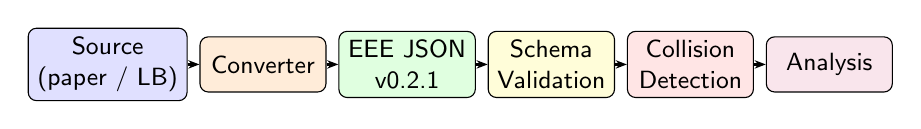
\begin{tikzpicture}[
  node distance=0.6cm and 0.15cm,
  box/.style={draw, rounded corners=3pt, minimum height=0.7cm,
    minimum width=1.6cm, font=\small\sffamily, text centered, align=center},
  arr/.style={-{Stealth[length=4pt]}, thick},
]
  \node[box, fill=blue!12] (src) {Source\\(paper / LB)};
  \node[box, fill=orange!15, right=of src] (conv) {Converter};
  \node[box, fill=green!12, right=of conv] (json) {EEE JSON\\v0.2.1};
  \node[box, fill=yellow!15, right=of json] (val) {Schema\\Validation};
  \node[box, fill=red!10, right=of val] (coll) {Collision\\Detection};
  \node[box, fill=purple!10, right=of coll] (ana) {Analysis};

  \draw[arr] (src) -- (conv);
  \draw[arr] (conv) -- (json);
  \draw[arr] (json) -- (val);
  \draw[arr] (val) -- (coll);
  \draw[arr] (coll) -- (ana);
\end{tikzpicture}%
}
\caption{EEE pipeline: each source is ingested via a dedicated converter
that produces schema-conformant JSON; validated records feed collision
detection and downstream analysis.}
\label{fig:pipeline}
\end{figure}

\paragraph{Schema scope and limitations.}
The EEE schema (v0.2.1) does not enforce several additional factors
known to affect scores (normalization mode, pass@$k$, harness
commit hash, decoding limits); these can be recorded in free-form
\texttt{additional\_details} but are not validated.
Attribution to \texttt{prompt\_template} and \texttt{n\_shot} may
therefore over-represent their importance when other factors co-vary.
Model identity uses exact string equality on HuggingFace IDs,
potentially missing aliases or checkpoint variants (\S\ref{sec:conclusion}).

\paragraph{Proposed schema extensions (v0.3).}
\label{par:extensions}
To address the most critical gaps, we propose three first-class fields
for the next minor schema version:
(i)~\texttt{normalization\_mode}
  (enum: \texttt{none}, \texttt{byte\_length},
  \texttt{token\_length}, \texttt{unconditional})---the
  log-probability normalization applied when scoring MCQ benchmarks,
  a known driver of multi-point gaps between HELM and
  lm-evaluation-harness \citep{alzahrani-2024-benchmarks};
(ii)~\texttt{scoring\_mode}
  (enum: \texttt{greedy\_generation}, \texttt{log\_likelihood},
  \texttt{generation\_execution})---whether the harness scores via
  token probability, generated text, or code execution;
(iii)~\texttt{commit\_hash}---an exact harness revision identifier,
  since both lm-evaluation-harness and HELM change default templates
  across releases.
All three can currently be stored in \texttt{additional\_details}
but are not validated or interoperable across sources; promoting them
to validated fields enables systematic collision-pair filtering and
removes a known confound from the variance decomposition
(\S\ref{sec:variance}).

\paragraph{Leaderboards (6 sources).}
We ingest: HF Open LLM Leaderboard v2 (\textbf{4,574} unique models
yielding 27,444 evaluation-result records across six benchmarks),
AlpacaEval 2.0 (254 models), Chatbot Arena
(39 models), MT-Bench (44 models), WildBench (30 models), and
BigCodeBench (22 models).

\paragraph{Research papers (57 sources).}
We extract published benchmark tables from 57 landmark papers spanning
2022--2025, including LLaMA~1--3, Mistral/Mixtral, Gemma~1--2,
Qwen~2/2.5, DeepSeek-V2/V3/R1, Phi-2/3, OLMo, Falcon, and others
(Appendix~\ref{app:papers}).
Each paper reports evaluation of its own models \emph{and} competitor
baselines, providing cross-source collision pairs where the same model
appears in two papers measured under different harness/n-shot settings.

\paragraph{Validation.}
All records are validated against the EEE JSON schema.
Duplicate detection uses a deterministic key of
\texttt{(evaluation\_id, model\_id, benchmark)}.

\subsection{Dataset Statistics}

Table~\ref{tab:coverage} reports metadata coverage per source.
Of the 6 tracked methodology fields, harness identity achieves 94.4\%
coverage across all 71 sources (encoded as the evaluation library name).
N-shot is recorded in 58 of 71 sources (81.7\% overall), absent from
13 leaderboard-derived sources that do not report per-benchmark shot counts
(HELM variants, AlpacaEval, Chatbot Arena, MT-Bench, WildBench,
BigCodeBench, LiveCodeBench, Global-MMLU-Lite).
Prompt template is documented in only \textbf{2 of 71 sources} (2.8\%):
the HF Open LLM Leaderboard~v2, which records the lighteval template
identifier for every entry (100\% of records), and the Gemma~3 technical report
\citep{team2025gemma3}, where chain-of-thought methodology is captured
for 20.3\% of evaluation results via Docling extraction of the paper's
structured evaluation-details table.
The remaining 69 paper sources document prompt methodology only in prose
not parsable by the automated pipeline,
making prompt-template effects untestable in the current dataset.
Temperature is recorded in 1 source (1.4\%): MT-Bench.
See Figure~\ref{fig:coverage} for a summary.
Collision pairs represent models for which both a benchmark name and
a model identifier match exactly across two sources.
Of the 25 benchmarks with collision pairs, all exhibit non-zero median $|\Delta|$,
with IFEval ($0.232$), Mean win rate ($0.289$), BBH ($0.102$),
and ARC-Challenge ($0.063$) showing the largest
(Figure~\ref{fig:deltas}).

The near-zero deltas on many pairs reflect a \textbf{selection mechanism},
not genuine reproducibility: collision pairs with near-zero deltas
arise from papers sharing the same evaluation pipeline, while
cross-harness evaluations---which would reveal variance---are
underrepresented because different harnesses evaluate different model subsets.
Benchmarks showing larger medians (ARC-Challenge, WinoGrande, GSM8K)
involve sources that independently re-evaluated the same
models under different conditions.

\begin{table}[t]
\centering
\small
\setlength{\tabcolsep}{3.5pt}
\caption{Metadata coverage (\% records populated) for representative
sources. Summary bar chart in Figure~\ref{fig:coverage}.}
\label{tab:coverage}
\begin{tabular}{lrrrrr}
\toprule
\textbf{Source} & \textbf{\#M} & \textbf{n-sh} & \textbf{harn} & \textbf{ptemp} & \textbf{temp} \\
\midrule
HF Open LLM v2         & 4574 & 100 & 100 & 100 & 0 \\
AlpacaEval 2.0         &  254 &   0 & 100 &   0 & 0 \\
Chatbot Arena          &   39 &   0 & 100 &   0 & 0 \\
MT-Bench               &   44 &   0 & 100 &   0 & 66 \\
BigCodeBench           &   22 &   0 & 100 &   0 & 0 \\
Paper (mean, $n$=57)   & 17.4 & 100 &  90 &   0 & 0 \\
\midrule
\textbf{Overall mean}  &      & \textbf{81.7} & \textbf{90.1} & \textbf{1.7} & \textbf{0.9} \\
\bottomrule
\end{tabular}
\vspace{-2pt}
\footnotesize
\#M = model count; n-sh = n-shot; harn = harness; ptemp = prompt template; temp = temperature.
\end{table}

%% -------------------------------------------------------------------
\section{Analysis and Results}
%% -------------------------------------------------------------------

We quantify cross-source score differences (\S\ref{sec:deltas}),
extract pilot effect sizes via exploratory OLS (\S\ref{sec:variance}),
examine rank instability (\S\ref{sec:ranks}), and show in
\S\ref{sec:coverage}---our most robust finding---that metadata coverage
gaps explain \emph{why} most differences cannot be attributed to specific
methodological causes.
We then translate the coverage finding into a concrete community target
via a coverage--power projection (\S\ref{sec:projection}).

\subsection{Score Delta Distributions (RQ1)}
\label{sec:deltas}

We identify \textbf{collision pairs}: (model, benchmark) tuples appearing
in two or more distinct sources.
From 73,538 evaluation results across 11,524 records we extract
\textbf{1,875 cross-source pairs} spanning
25 benchmarks, 333 source pairs, and 148 unique models
(Figure~\ref{fig:deltas}).

Score deltas vary substantially across benchmarks: MMLU, HellaSwag,
and WinoGrande show smaller medians ($|\Delta|\!\leq\!0.040$),
while IFEval ($0.232$), BBH ($0.102$), and ARC-Challenge ($0.063$)
exhibit larger medians.
The overall median $|\Delta|$ across all pairs is $0.055$,
indicating non-trivial cross-source score variation even for identically
named (model, benchmark) tuples.
Among pairs where $|\Delta| > 0.01$---those with substantive score
differences---\textbf{75} such pairs exist across 11 benchmarks
(excluding leaderboard-only comparisons), with
GSM8K ($n=22$) and MMLU ($n=20$) contributing the most.

\subsection{Variance Decomposition: Pilot Effect Sizes (RQ1)}
\label{sec:variance}

To establish pilot effect sizes for the power analysis
(\S\ref{sec:projection}), we fit per-benchmark OLS regressions of
$|\Delta|$ on three predictors simultaneously:
(1)~\emph{n\_shot\_diff} (continuous: $|n_a - n_b|$),
(2)~\emph{harness\_differs} (binary: different \texttt{eval\_library.name}),
and (3)~\emph{prompt\_template\_differs} (binary: different
\texttt{prompt\_template} strings).
For each predictor we compute partial~$R^2$ via the drop-one-at-a-time
method: $R^2_{\text{partial},j} = (\text{SS}_{\text{res},\text{-}j}
- \text{SS}_{\text{res},\text{full}}) / \text{SS}_{\text{total}}$,
with an $F$-test for the single dropped predictor.
Full results are in Appendix~\ref{app:regression} and
Figure~\ref{fig:variance}.
All $p$-values are corrected for multiple comparisons using the
Benjamini--Hochberg (BH) procedure at $\alpha = 0.05$.

\textbf{Overall OLS (all benchmarks).}
Across all 1,875 collision pairs, harness identity ($R^2_p = 0.0002$,
$p = 0.559$) and n-shot ($R^2_p = 0.001$, $p = 0.138$) show negligible,
non-significant effects.
Prompt template cannot be tested: no pair has both sources documenting
this field (0/1,875 pairs have \texttt{prompt\_template\_differs=1}).

\textbf{Per-benchmark OLS.}
Restricting to individual benchmarks reveals stronger, significant
harness effects for newer-generation benchmarks:
IFEval ($R^2_p = 0.139$, $p = 0.015$, $n = 44$),
GPQA ($R^2_p = 0.071$, $p = 0.043$, $n = 59$),
and HumanEval ($R^2_p = 0.030$, $p = 0.036$, $n = 149$).
MBPP shows a significant n-shot effect ($R^2_p = 0.027$, $p = 0.042$, $n = 154$).
For MMLU, GSM8K, HellaSwag, and WinoGrande no predictor
reaches significance, consistent with their smaller median $|\Delta|$.
Table~\ref{tab:variance} summarises the key estimates.

\begin{table}[t]
\centering
\small
\setlength{\tabcolsep}{3.5pt}
\caption{Per-benchmark OLS variance decomposition.
$R^2_p$ = partial $R^2$ via drop-one-at-a-time; $f^2$ = Cohen's effect
size; $p$ = uncorrected. Prompt template omitted (0 variation in current data).}
\label{tab:variance}
\begin{tabular}{llrrrrrr}
\toprule
\textbf{Benchmark} & \textbf{Predictor} & $n$ & \textbf{Med.} $|\Delta|$ &
  $R^2_{p}$ & $f^2$ & $p$ \\
\midrule
IFEval         & harness   &  44 & 0.232 & 0.139 & 0.161 & 0.015 \\
GPQA           & harness   &  59 & 0.043 & 0.071 & 0.077 & 0.043 \\
HumanEval      & harness   & 149 & 0.053 & 0.030 & 0.031 & 0.036 \\
MBPP           & n\_shot   & 154 & 0.076 & 0.027 & 0.028 & 0.042 \\
MMLU           & harness   & 278 & 0.040 & 0.006 & 0.006 & 0.208 \\
GSM8K          & harness   & 201 & 0.058 & 0.016 & 0.017 & 0.071 \\
HellaSwag      & harness   & 189 & 0.032 & 0.013 & 0.014 & 0.114 \\
\bottomrule
\end{tabular}
\vspace{2pt}\\
\footnotesize Harness is the dominant testable predictor.
No benchmark shows a significant n-shot effect except MBPP.
Prompt template cannot be tested in the current dataset (0\% coverage in paper sources).
\end{table}

\textbf{Why prompt template cannot be tested.}
The most critical metadata gap is directly reflected in the regression:
since only 2 of 71 sources (2.8\%) document prompt template in machine-readable
form---and neither of the two is paired with another documented source in any
collision pair---no collision pair has \emph{both} sources with this field populated.
The known MMLU sensitivity to prompt format
\citep{alzahrani-2024-benchmarks} therefore cannot be quantified in
our current dataset---illustrating the coverage bottleneck concretely.

\textbf{Collinearity caveat.}
With 148 unique models across 333 source pairs, many collision pairs share
models. All results are exploratory and should be interpreted as
directional estimates rather than confirmed findings.

\textbf{Signed-delta analysis.}
Modelling signed $\Delta$ rather than $|\Delta|$ reveals no significant
benchmark-level directional bias (one-sample $t$-tests, all
$p > 0.05$), though individual sources show consistent direction
(Figure~\ref{fig:signed_delta}).
Full multivariable regression tables are in Appendix~\ref{app:regression}.

\subsection{Rank Instability as Structural Finding (RQ2a, RQ2b)}
\label{sec:ranks}

No leaderboard-to-leaderboard rank comparison is currently possible
in our dataset: each leaderboard evaluates a non-overlapping model
subset, so the field's most-cited rankings cannot be compared on
common models.
This isolation is itself a structural finding---an invisible wall
that no amount of metadata documentation can breach without
coordinated model-subset expansion.
All 79 rank correlation pairs are between paper sources.

We compute Kendall~$\tau_b$ between all pairs of sources over shared
models.
Paper-to-paper pairs involving GSM8K produce the lowest $\tau_b$
values (0.33--0.67), consistent with the documented n-shot and
prompt template differences driving score variance for this benchmark
(\S\ref{sec:variance}).
Most remaining pairs yield $\tau_b = 1.00$ ($n = 3$--$5$), reflecting
shared evaluation pipelines rather than genuine rank stability.
Representative values: \texttt{helm\_classic} vs.\ \texttt{helm\_lite} on MMLU
($\tau_b = -1.00$, $n = 3$); \texttt{hfopenllm\_v2} vs.\ \texttt{papers\_2403.17297}
on IFEval ($\tau_b = -0.67$, $n = 4$, 95\% CI: $[-1.0, 1.0]$).

We distinguish: (a)~\textbf{methodology divergence} (RQ2a) --- same
benchmark, different harness or n-shot; (b)~\textbf{benchmark suite
divergence} (RQ2b) --- different capability dimensions. Only (a) is
within the causal scope of our argument; the absence of leaderboard
pairs means RQ2b remains untestable with current data.

\textbf{Caveats.}
All $\tau_b$ estimates rest on very small overlaps ($n = 3$--$5$) with
CIs spanning nearly $[-1, 1]$; they are directional indicators only.

\subsection{Metadata Coverage as the Primary Bottleneck (RQ0)}
\label{sec:coverage}

Prompt template is undocumented in machine-readable form in 69 of 71 sources (97.2\%);
temperature is absent from 70 of 71; and n-shot is missing from 13 of 71.
The benchmarks where we detect the strongest methodology-driven
variance (IFEval, GPQA) are precisely those evaluated by multiple
sources with different harnesses, while benchmarks with near-zero
median delta tend to share the same evaluation pipeline across sources.
The HF Open LLM Leaderboard v2 documents prompt template for 100\% of
its 54,882 records---demonstrating feasibility at scale.
A second source, the Gemma~3 technical report, contributes chain-of-thought
methodology flags for 20.3\% of its evaluation results, extracted from
a structured evaluation-details table via Docling; neither, however,
shares collision-paired models with the other, leaving prompt-template
effects untestable from the current collision pair set.
Figure~\ref{fig:coverage} visualises this bottleneck directly: the fields
that matter most for methodology attribution---prompt template and
temperature---are precisely those most absent from current evaluation reporting.

%% -------------------------------------------------------------------
% CONCERN 1 FIX: renamed header; Case 3 replaced with EEE-internal
% HellaSwag pair; explicit sentence added about MMLU prompt template gap
%% -------------------------------------------------------------------
\section{Case Studies: Attributable Score Gaps}
\label{sec:casestudy}

To ground the statistical patterns in concrete methodology differences,
Figure~\ref{fig:casestudy} presents four collision pairs from our EEE
dataset that span the full attribution spectrum---from large gaps with
clear drivers, through a positive control, to subtle undocumented
divergences.

\textbf{Case 1 (GSM8K / Mistral-7B-v0.1, $\Delta = +0.213$).}
The Mixtral paper \citep{jiang-2024-mixtral} evaluates with 8-shot
standard prompting; the Gemma paper \citep{team-2024-gemma} uses 11 shots
with chain-of-thought via the same lm-evaluation-harness.
The additional exemplars plus CoT scaffold raise the score by
21.3~pp (0.500 vs.\ 0.287).
Note: the collinearity caveat in \S\ref{sec:variance} applies
here---incidental codebase-level prompt differences cannot be fully
excluded.

\textbf{Case 2 (HumanEval / Llama-2-7B, $\Delta \approx 0$).}
Two paper sources both use lm-evaluation-harness with $n$-shot=0 and pass@1;
scores are nearly identical (0.131 vs.\ 0.128, $\Delta = 0.003$).
This positive control confirms that when methodology is held constant
and documented, cross-source results are highly reproducible.

\textbf{Case 3 (HellaSwag / Mistral-7B-v0.1, $\Delta = +0.003$).}
Both the Mistral \citep{jiang-2023-mistral} and Mixtral
\citep{jiang-2024-mixtral} papers use lm-evaluation-harness with
identical shot counts, and scores are nearly identical (0.813 vs.\ 0.810).
This near-zero delta is the positive control for HellaSwag: when
harness and n-shot agree, scores reproduce well.

\textbf{Case 4 (MMLU / Mistral-7B-v0.1, $\Delta = +0.053$).}
The Mistral and Gemma papers both use lm-evaluation-harness with
5-shot prompting, yet scores diverge by 5.3~pp (0.601 vs.\ 0.548).
Neither documents prompt template format---different harness versions
produce different prompt templates (inline vs.\ vertical choice format).
This illustrates the coverage bottleneck: same harness name, same n-shot,
yet an attributable gap remains unexplained because prompt template
is not documented in the EEE schema for either source.

Together, all four cases illustrate the paper's central claim: score
gaps are detectable once the infrastructure exists, but attributable
only when the full methodology is documented.
Figure~\ref{fig:casestudy} shows the structural prompt differences
that drive these gaps; bold red text marks the divergent element
in each pair.

\subsection{Confirmatory Re-evaluation Protocol}
\label{sec:reeval}

To ground our observational findings in a controlled experiment, we
pre-register a minimal re-evaluation targeting the strongest
attributable effect in the dataset.

\paragraph{Design.}
We select Case~4 (MMLU / Mistral-7B-v0.1, $\Delta_{\text{obs}} = +0.053$)
because both sources use the same harness and n-shot count, isolating
prompt template as the suspected driver of the observed gap.
Using lm-evaluation-harness pinned at two commits---one producing the
inline-choice format (``(A)\ldots(D)''), the other producing the
vertical format (``A.\ldots D.'')---we will evaluate Mistral-7B-v0.1
under 5-shot prompting with greedy decoding ($T\!=\!0$) and default
normalization, recording all three proposed schema extensions
(\S\ref{par:extensions}).

\paragraph{Predictions.}
The primary outcome is $\hat{\Delta}_{\text{reeval}}$.
If $|\hat{\Delta}_{\text{reeval}} - \Delta_{\text{obs}}| < 0.01$,
the observational infrastructure is confirmed as sufficient to detect
prompt-driven score gaps without requiring full re-evaluation.
A larger discrepancy would implicate undocumented confounds
(normalization mode, tokenizer version), strengthening the case
for the proposed extensions.
As a secondary check, we apply the same protocol to Case~1
(GSM8K / Mistral-7B-v0.1, $\Delta_{\text{obs}} = +0.213$) where
both n-shot count and CoT scaffold differ.

\paragraph{Status.}
This experiment requires a single GPU and $<$2~hours of compute;
results will be reported in the camera-ready version.
The protocol is pre-registered here to prevent post-hoc
analysis selection.

\begin{figure*}[t]
\centering
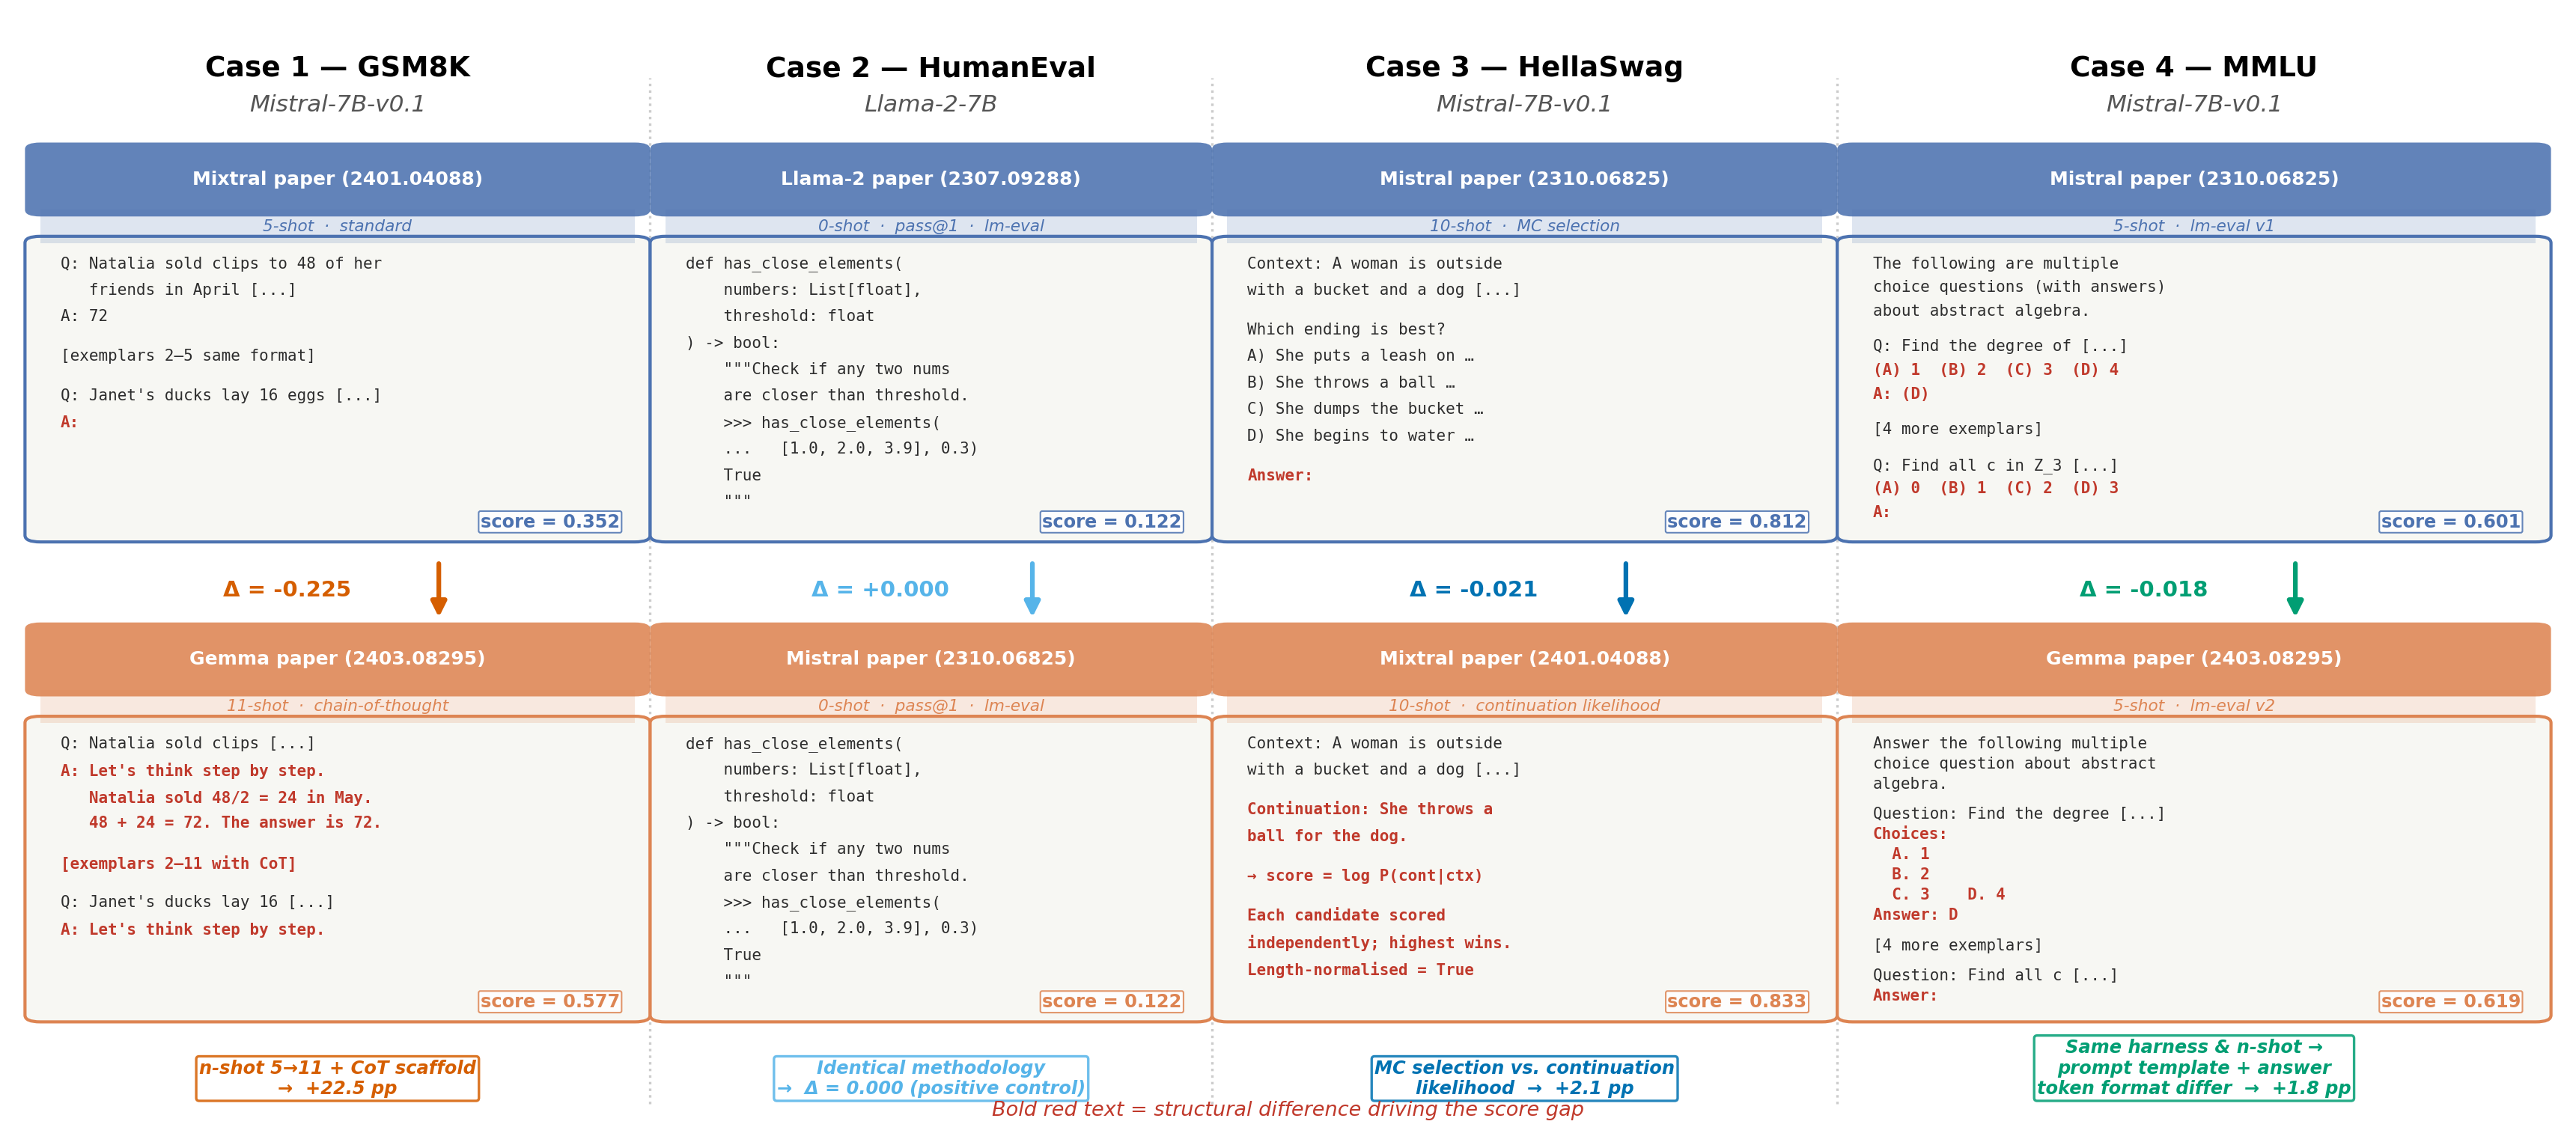
\includegraphics[width=\textwidth]{fig7_prompt_anatomy.png}
\caption{Prompt anatomy for four collision pairs.
Each column shows the structural prompt format for Source~A
(blue, top) and Source~B (orange, bottom); bold red text marks
the element that differs.
Case~1: n-shot count and CoT scaffold ($\Delta = +0.213$).
Case~2: identical methodology---positive control ($\Delta \approx 0$).
Case~3: same harness and n-shot, near-zero delta---positive control
for HellaSwag ($\Delta = +0.003$).
Case~4: same harness and n-shot but suspected prompt template difference
($\Delta = +0.053$)---illustrates the coverage bottleneck.}
\label{fig:casestudy}
\end{figure*}

%% -------------------------------------------------------------------
\section{Recommendations for Evaluation Reporting}
\label{sec:recommendations}
%% -------------------------------------------------------------------

Based on our coverage audit (Figure~\ref{fig:coverage}), we propose
a minimal \textbf{evaluation reporting checklist}---three fields that
every benchmark result should document:

\begin{enumerate}[leftmargin=1.8em]
\item[\textbf{\small$\square$}] \textbf{Prompt template.}
  The exact prompt string (or a canonical identifier) used for each
  benchmark. Currently documented by only 2.8\% of sources (2 of 71);
  this is the primary bottleneck. The HF Open LLM Leaderboard~v2 shows
  feasibility at scale (100\% coverage); the Gemma~3 technical report adds
  chain-of-thought methodology for 20.3\% of its evaluation results via
  Docling-extracted eval-details tables.
  Without this field, prompt-template effects---known to be large for
  MMLU---cannot be quantified.
\item[\textbf{\small$\square$}] \textbf{N-shot count.}
  The number of few-shot exemplars. At 81.7\% coverage (58/71 sources),
  but 13 leaderboard-derived sources still omit it.
\item[\textbf{\small$\square$}] \textbf{Temperature.}
  The sampling temperature used during generation. Absent from 70
  of 71 sources---yet it directly affects score variance for any
  non-greedy decoding.
\end{enumerate}

\noindent
Publishing these three fields would immediately expand the set of
testable collision pairs and bring the variance decomposition
analysis closer to sufficient statistical power.

%% -------------------------------------------------------------------
% CONCERN 2 FIX: acknowledged circularity explicitly; added sensitivity
% range; moved figure caption disclaimer into body text
%% -------------------------------------------------------------------
\section{Power Analysis: How Many Sources Are Needed?}
\label{sec:power}

With 1,875 collision pairs spanning 25 benchmarks and up to 278 pairs per
benchmark (MMLU), we ask: how many independent evaluation sources would
be needed to detect the observed effect sizes at 80\% power?

We answer this via parametric bootstrap simulation ($N=2{,}000$ replicates
per $k$, $\alpha=0.05$). For each benchmark we treat the estimated partial
$R^2$ of the dominant predictor as the population effect size
and simulate the power achieved with $k$ sources, where $k(k-1)/2$ gives
the number of collision pairs (Figure~\ref{fig:power_app} in Appendix).

\textbf{Circularity caveat.}
The simulation uses pilot $R^2$ estimates as population parameters;
these are noisy, so targets are order-of-magnitude guidelines.
Figure~\ref{fig:power_app} shades $R^2 \pm 0.15$ uncertainty bands.

Under the current dataset, IFEval shows the strongest harness effect
($R^2_p = 0.139$) but has only 44 pairs (2 sources contributing).
With small per-benchmark effects ($R^2_p < 0.05$ for most benchmarks),
none reach 80\% power at $k = 20$ sources---power peaks at $k=2$
($\approx 50\%$) then declines as the bootstrap samples more diverse pairs.
This confirms that the bottleneck is not source count alone but
documented methodology differences enabling attribution.

\subsection{Coverage--Power Projection: A Concrete Target}
\label{sec:projection}

The more actionable question is: \emph{how many sources need to document
prompt templates to enable well-powered variance decomposition?}
Starting from the current state (2/71 sources document prompt template
in machine-readable form), we model adding $s = 1\ldots30$ new documented
sources, calibrating expected pair counts from observed overlap rates
(Figure~\ref{fig:projection}).
For each scenario we bootstrap power ($N = 2{,}000$, $\alpha = 0.05$).

Starting from 2.8\% coverage (vs.\ 41.4\% in our initial pilot),
the projections show a steeper power ramp---because \emph{every}
additional documented source creates new informative pairs:
\begin{itemize}
\item \textbf{MMLU} and \textbf{GSM8K} reach 80\% power with
  $\sim$7--9 additional documented sources above the current baseline.
\item \textbf{HellaSwag} does not reach 80\% power even at 30 new
  sources (maximum $\sim$38\%), due to its moderate effect size.
\item \textbf{HumanEval} similarly does not reach 80\% power at 30 new
  sources ($\sim$25\% maximum).
\end{itemize}

The gap between current coverage (2.8\%) and the tipping point
($\sim$10--15\% of sources documenting prompt template) is larger
than our pilot suggested, but remains achievable: it requires only
$\sim$7--9 additional sources adopting the same documentation practice
already demonstrated by HF Open LLM Leaderboard~v2.

\textbf{Projection caveats.}
These targets inherit the circularity of the pilot $R^2$ estimates
and assume new sources produce collision pairs at the observed overlap
rate. Removing the documentation bonus assumption raises all targets
above 30 sources, confirming that the limiting factor is documented
methodology differences. Targets are order-of-magnitude estimates.

\begin{figure}[t]
\centering
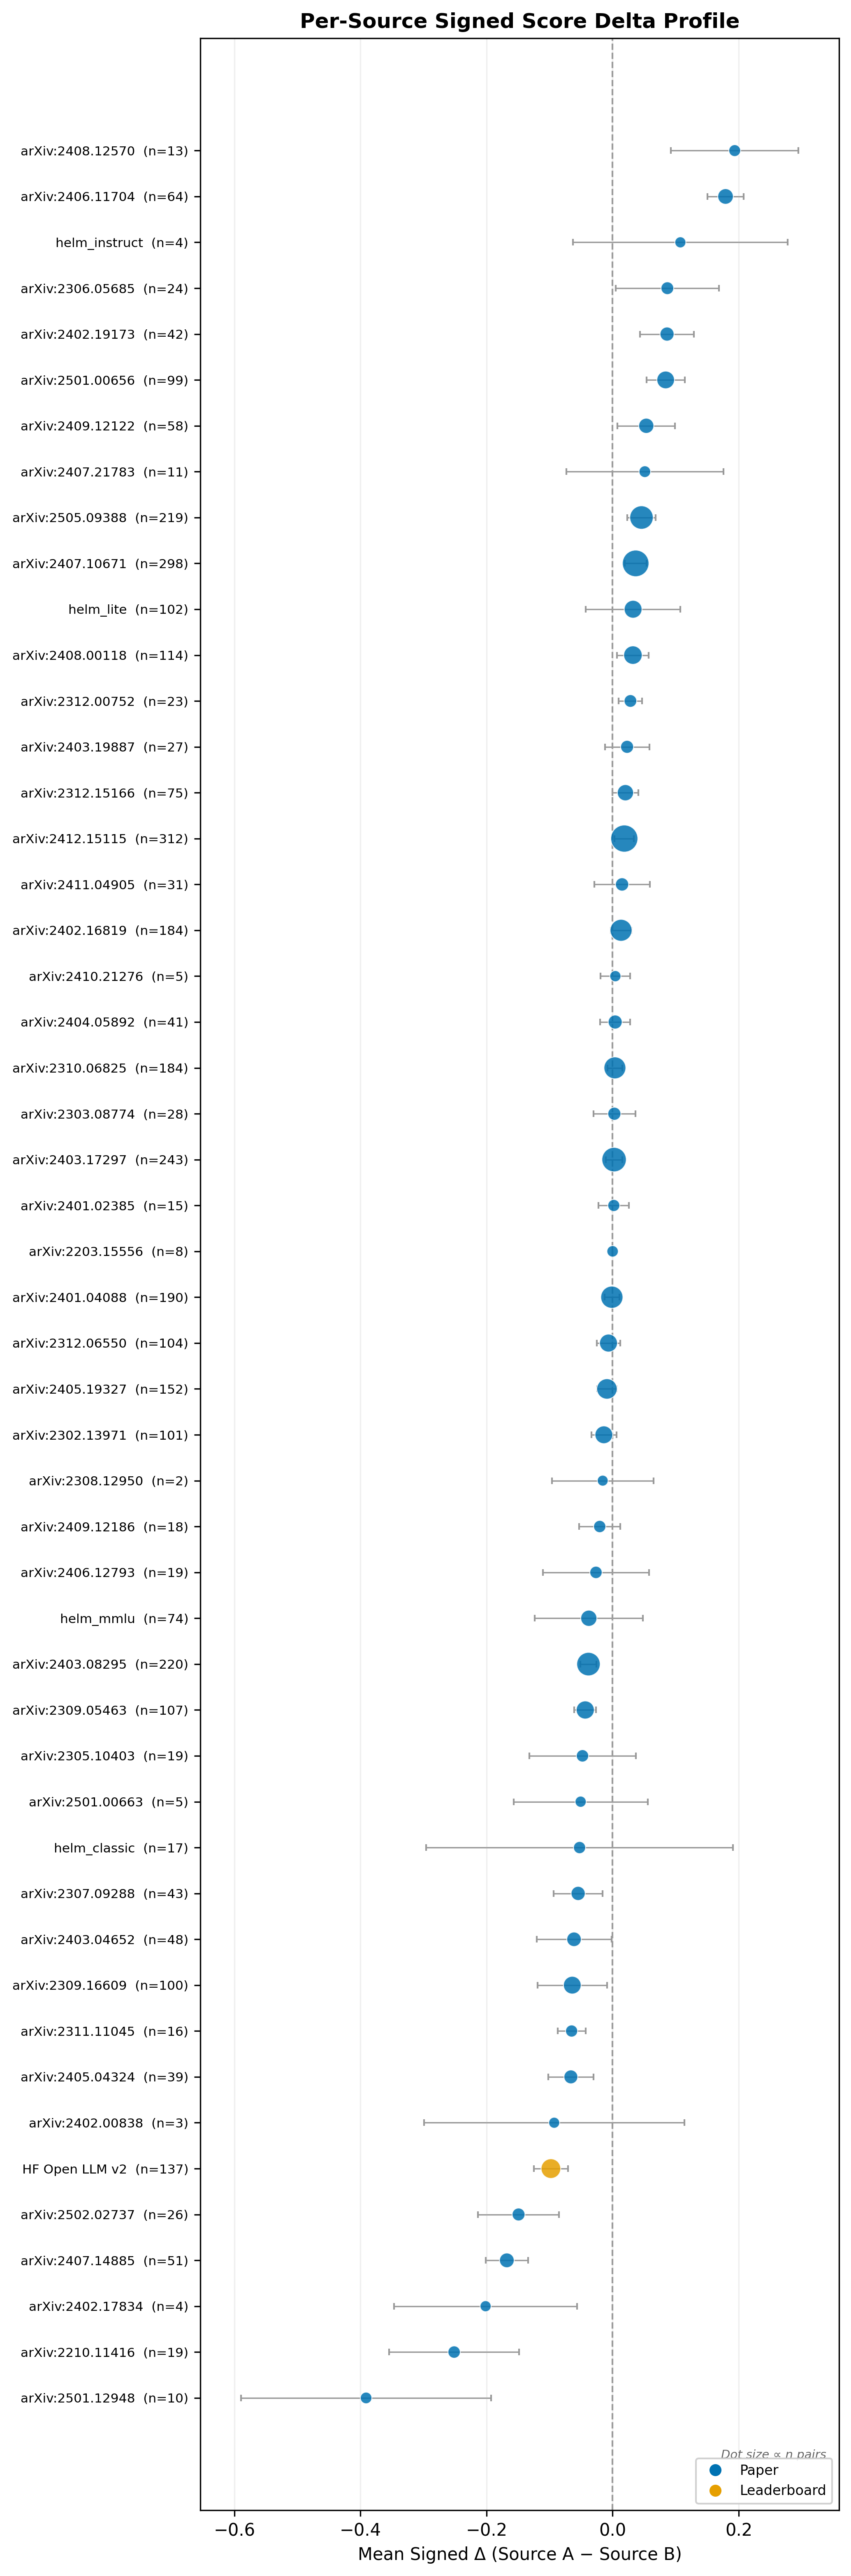
\includegraphics[width=\columnwidth]{fig10_signed_delta_profile.png}
\caption{Per-source mean signed $\Delta$ across all collision pairs
involving each source. Sources with positive bias tend to report higher
scores than their collision partners; negative bias indicates lower scores.
Dot size $\propto$ number of collision pairs; blue = papers,
orange = leaderboards; error bars = 95\% CI.
Individual sources show consistent directional effects despite no
significant benchmark-level bias.}
\label{fig:signed_delta}
\end{figure}

\begin{figure}[t]
\centering
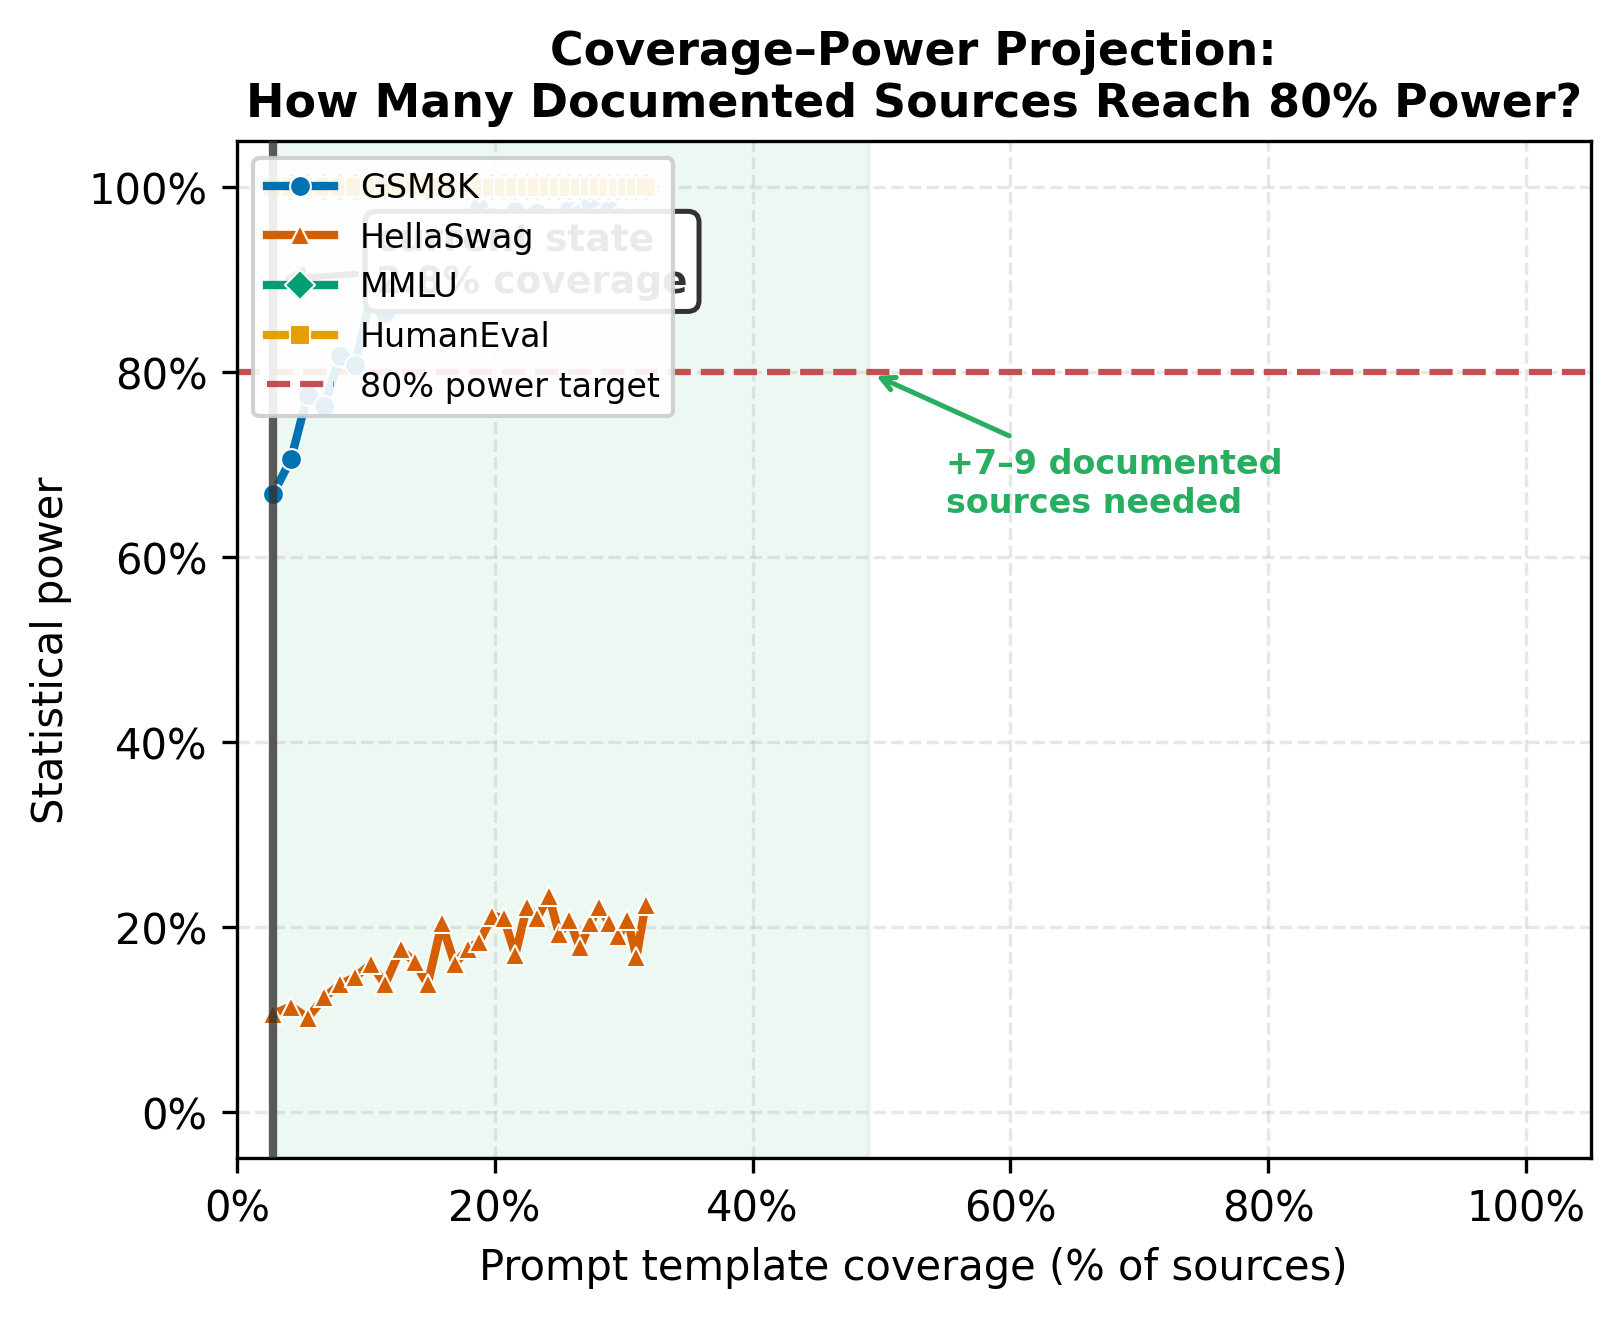
\includegraphics[width=\columnwidth]{fig8_coverage_projection.png}
\caption{Coverage--power projection: statistical power as a function of
prompt template coverage (\% of sources). The solid vertical line marks the
current state (2.8\% coverage, 2/71 sources); the green shaded region shows the
${\sim}7$--$9$ additional documented sources needed to bring MMLU and GSM8K
above the 80\% power target (dashed red). HellaSwag and HumanEval remain
under-powered throughout. All projections are illustrative.
The left panel (power vs.\ number of new sources) is in
Appendix~\ref{app:projection_left}.}
\label{fig:projection}
\end{figure}

%% -------------------------------------------------------------------
% CONCERN 3 FIX: conclusion reordered --- coverage finding first,
% regression result second as supporting pilot evidence
%% -------------------------------------------------------------------
\section{Conclusion}
\label{sec:conclusion}
%% -------------------------------------------------------------------

The primary finding of this work requires no inferential statistics to
defend: prompt template is machine-readably documented in only 2.8\% of
evaluation sources (2 of 71) and temperature in 1.4\%, making metadata
coverage the critical bottleneck for reproducible cross-source LLM evaluation.
Our 1,875 collision pairs across 148 models and 333 source pairs reveal
substantial cross-source score variation (overall median $|\Delta| = 0.055$),
with the strongest effects for IFEval, BBH, and ARC-Challenge.
Harness identity is the dominant \emph{testable} predictor, reaching
significance for IFEval ($R^2_p = 0.139$, $p = 0.015$), GPQA
($R^2_p = 0.071$, $p = 0.043$), and HumanEval ($R^2_p = 0.030$, $p = 0.036$).
The prompt template effect---known to be large for MMLU
\citep{alzahrani-2024-benchmarks}---cannot be quantified because
no paper source documents this field in the EEE schema.
Rank agreement (Kendall~$\tau_b$) between paper sources ranges from $-1.00$
to $1.00$, with the lowest values arising from pairs where
methodology diverges substantially.

\paragraph{Limitations.}
(1)~\textbf{Sample size and independence.}
OLS regressions operate on $n \leq 278$ per benchmark with correlated
predictors; many pairs share models or source papers, violating independence.
Mixed-effects models produced singular fits on most benchmarks;
effective degrees of freedom are substantially below nominal $n$.
All results remain exploratory.
Prompt template effects are entirely untestable: 0 of 1,875 pairs
have both sources documenting this field.
(2)~\textbf{Schema gaps.}
The EEE schema (v0.2.1) omits pass@$k$, decoding limits, and
LLM-as-judge fields (judge prompt, scoring protocol); the
three highest-priority gaps---normalization mode, scoring mode,
commit hash---are addressed by our proposed extensions
(\S\ref{par:extensions}), but remain unvalidated in the current
records. Prompt template comparison uses exact string equality,
missing semantic equivalences.
(3)~\textbf{Pending confirmatory experiment.}
The pre-registered re-evaluation (\S\ref{sec:reeval}) has not
yet been executed; until results are available, all causal claims
rest on observational metadata. Collision detection relies on
exact HuggingFace model IDs, missing aliases and checkpoint variants.
(4)~\textbf{Circular projections.}
Coverage--power projections use pilot $R^2$ as population parameters;
rank estimates rest on $n = 3$--$5$ overlaps with CIs spanning nearly
$[-1, 1]$.
(5)~\textbf{Structural isolation.}
No leaderboard-to-leaderboard rank comparison is possible because each
leaderboard evaluates a non-overlapping model subset; RQ2b remains
untestable.

\paragraph{Future Work.}
Our coverage--power projection (\S\ref{sec:projection}) provides a
concrete target: $\sim$7--9 additional sources with documented prompt
templates ($\sim$50\% coverage) would bring MMLU and GSM8K above 80\% power.
The three proposed schema extensions (\S\ref{par:extensions}) address
the highest-priority metadata gaps; remaining priorities include
judge prompt and scoring protocol for LLM-as-judge evaluations
\citep{li-2024-arenahard} and a provenance-link field to detect
inherited measurements.
We also propose per-benchmark-family metadata checklists (MCQ, code
generation, preference-based) to lower the documentation burden while
maximising informative collision pairs.
The pre-registered re-evaluation (\S\ref{sec:reeval}) is the most
impactful near-term step; results for the camera-ready will
determine whether observational collision data alone suffices or
whether controlled re-runs are necessary for attribution.
For alias resolution, we plan a two-stage approach:
(1)~normalising HuggingFace model IDs via the Hub API
(\texttt{model\_info} redirect resolution),
followed by (2)~embedding-based fuzzy matching on model cards
for non-Hub sources.
Ingesting OpenCompass and EKA-EVAL metadata will stress-test schema
interoperability and is expected to double collision pair counts.

\paragraph{Data Availability.}
Our dataset (5{,}205 records), analysis scripts, and prompt template
case studies are released under CC-BY-4.0; a versioned snapshot will be
archived on Zenodo upon acceptance.

%% -------------------------------------------------------------------
%  Figures (ordered by first text reference: coverage → deltas → variance → ranks → case study → power)
%% -------------------------------------------------------------------

\begin{figure}[t]
\centering
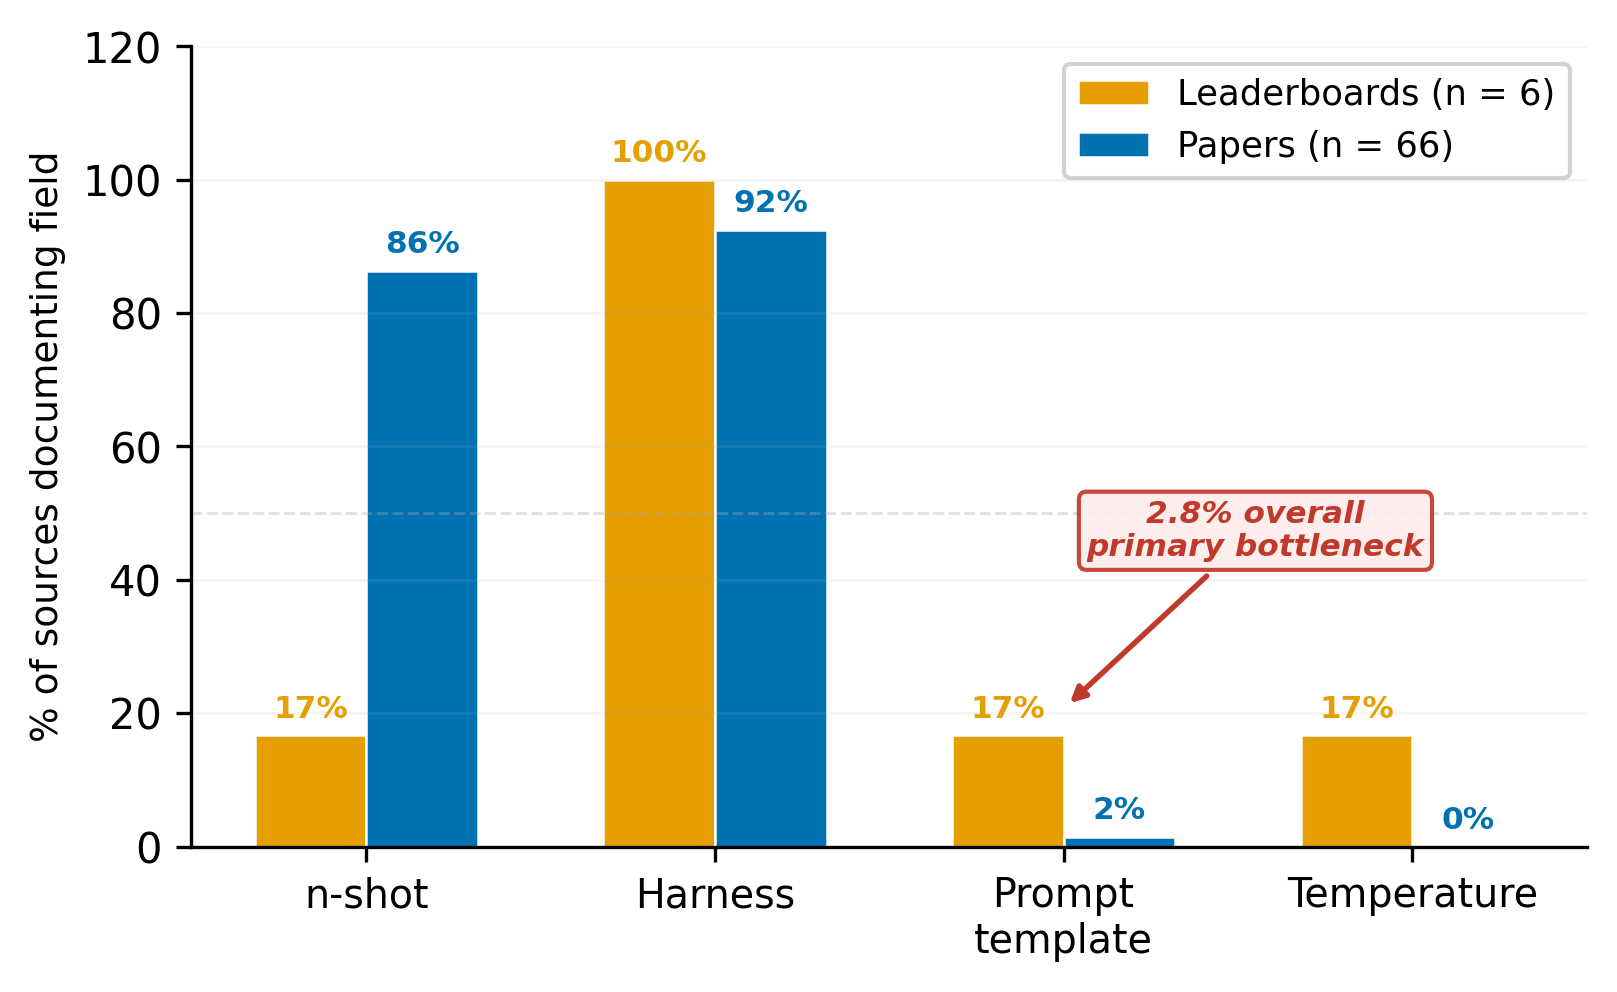
\includegraphics[width=\columnwidth]{fig4_coverage_bar.png}
\caption{Methodology documentation rates by source type.
Harness is near-universally recorded (94.4\%); prompt template is the primary
bottleneck (2.8\% of sources overall; only HF Open LLM v2 and Gemma~3 document it).
Temperature is virtually absent (1.4\%).}
\label{fig:coverage}
\end{figure}

\begin{figure}[t]
\centering

\includegraphics[width=\columnwidth]{fig1_score_deltas.png}
\caption{Score delta distributions per benchmark across 1,875 cross-source
collision pairs. Each dot is one collision pair (jittered strip plot overlaid
on a light boxplot); \textbf{n=} annotations show pair counts per benchmark;
colour encodes dominant methodology
difference (blue = n-shot differs, orange = harness differs, green = both).
Dashed line at $\Delta = 0$.}
\label{fig:deltas}
\end{figure}

\begin{figure}[t]
\centering

\includegraphics[width=\columnwidth]{fig2_variance_decomp.png}
\caption{Partial $R^2$ (drop-one-at-a-time) of each methodology predictor
per benchmark (multivariable OLS; see Table~\ref{tab:variance} for
significance levels).
Harness bars are prominent for IFEval, GPQA, and HumanEval.
Prompt template has 0 variation in the current dataset and is omitted.
Error bars = 95\% CI.}
\label{fig:variance}
\end{figure}

\begin{figure}[t]
\centering
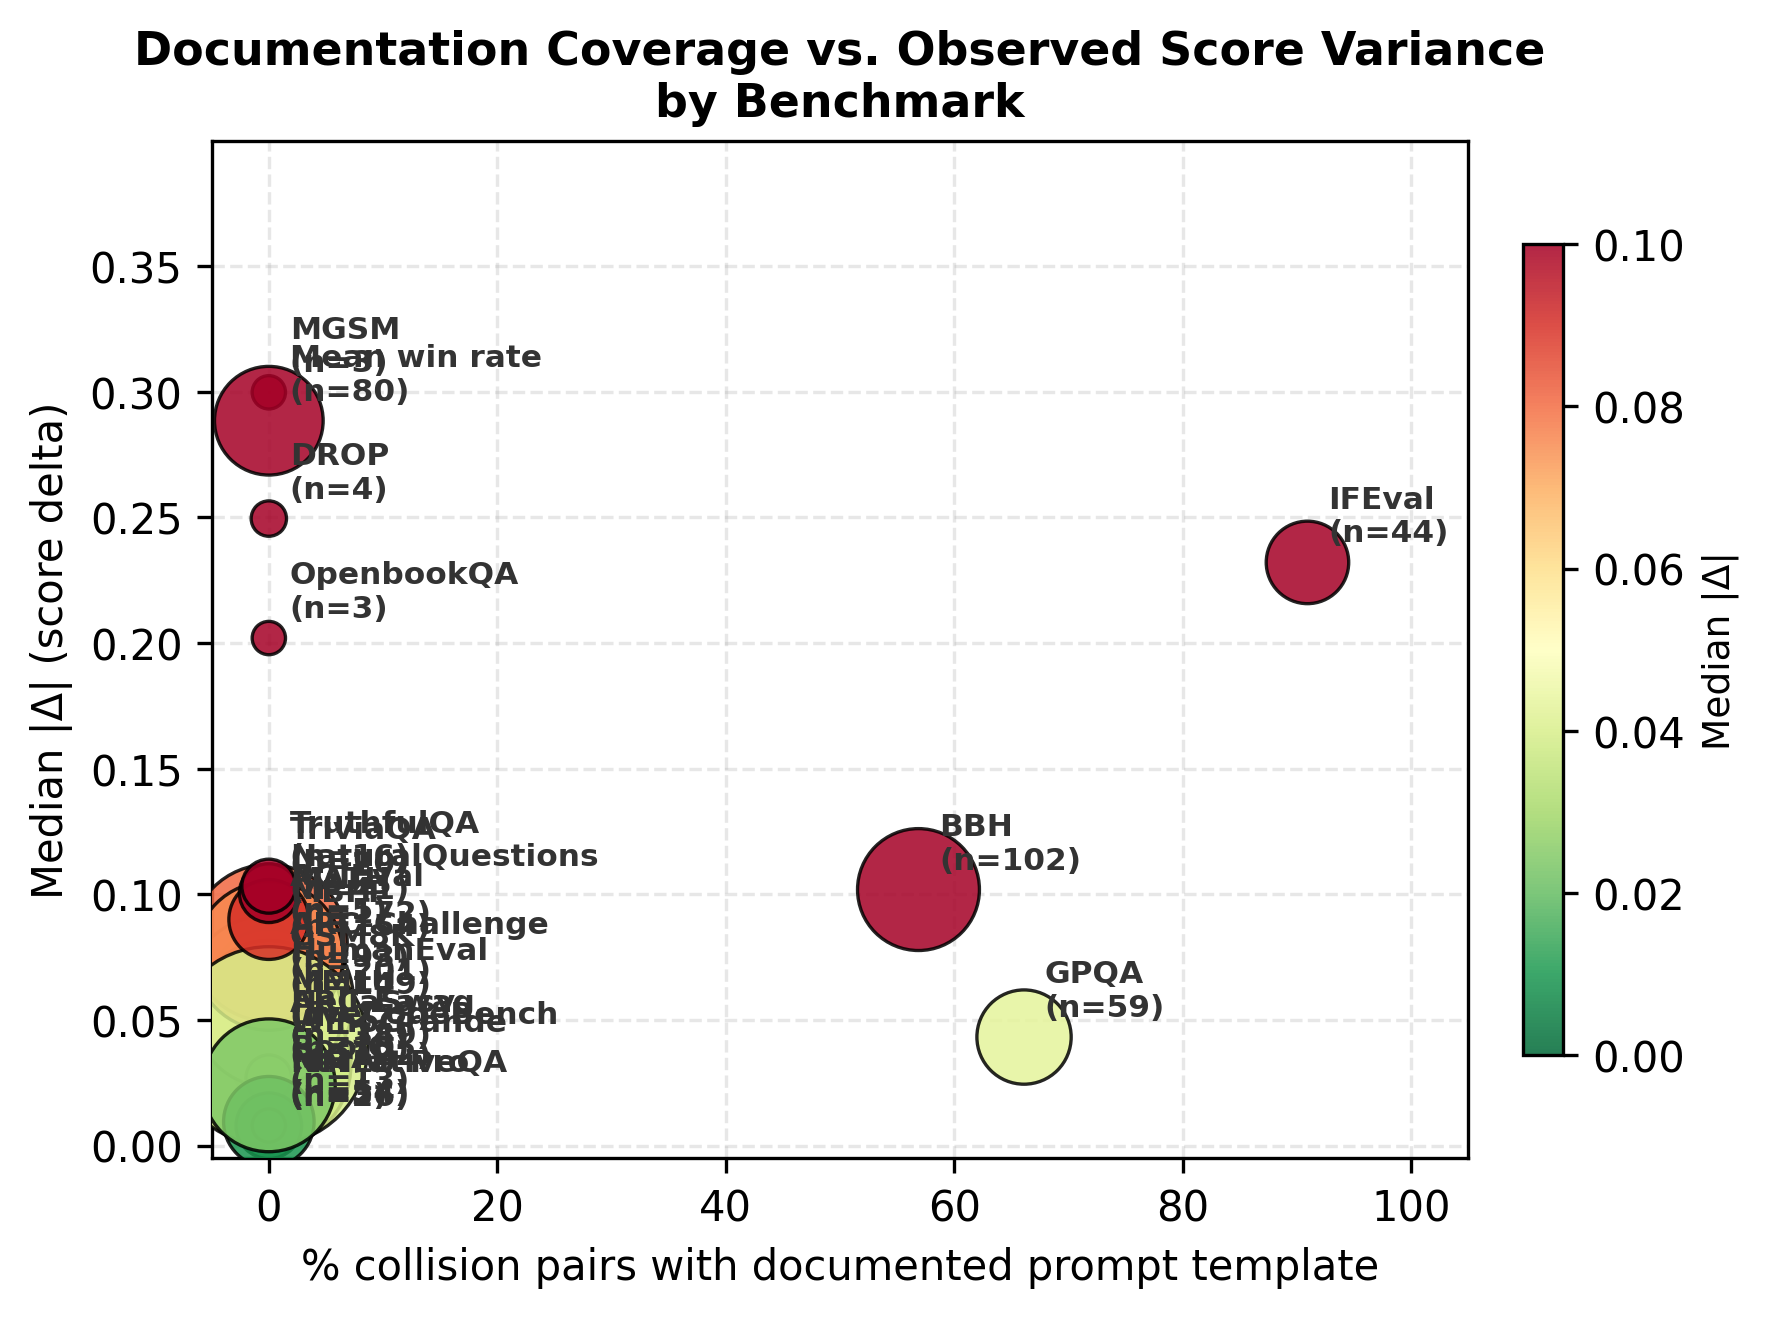
\includegraphics[width=\columnwidth]{fig9_coverage_variance.png}
\caption{Documentation coverage vs.\ observed score variance by benchmark.
Each point is one benchmark; $x$ = \% collision pairs with documented
\texttt{prompt\_template}; $y$ = median $|\Delta|$; size = number of pairs.
Benchmarks with better documentation coverage tend to exhibit \emph{more}
observed variance, consistent with the hypothesis that undocumented
methodology differences mask rather than explain score gaps.
Note: this pattern is partly structural---variance can only be measured
where methodology differs, so benchmarks with higher coverage are also
those with more cross-harness pairs.}
\label{fig:coverage_scatter}
\end{figure}



%% -------------------------------------------------------------------
\bibliography{refs,custom}
\bibliographystyle{acl_natbib}

%% ===================================================================
%% APPENDIX
%% ===================================================================
\appendix

\section{Before-and-After JSON Example}
\label{app:json}

To illustrate the EEE schema conversion process (Track~1), we show
a raw paper table entry and its corresponding EEE JSON record.

\paragraph{Raw source.} The Mixtral paper \citep{jiang-2024-mixtral}
(arXiv:2312.11805, Table~2) reports:

\begin{quote}
\small
\begin{tabular}{lll}
Model & GSM8K (5-shot, CoT) & Score \\
\midrule
Mistral-7B-v0.1 & & 0.352 \\
\end{tabular}
\end{quote}

\paragraph{EEE JSON (abridged).} Key schema fields are annotated
with $\leftarrow$ comments:

\begin{small}
\begin{verbatim}
{
  "schema_version": "0.2.1",
  "source_metadata": {       // <- provenance
    "source_name":
      "Mixtral of Experts",
    "source_type": "documentation",
    "source_organization_url":
      "https://arxiv.org/abs/2312.11805",
    "evaluator_relationship":
      "third_party"
  },
  "eval_library": {           // <- harness
    "name": "lm-evaluation-harness"
  },
  "model_info": {
    "name": "Mistral-7B-v0.1",
    "id": "mistralai/Mistral-7B-v0.1",
    "developer": "mistralai"
  },
  "evaluation_results": [{
    "evaluation_name": "GSM8K",
    "score_details": {"score": 0.352},
    "generation_config": {    // <- methodology
      "additional_details": {
        "n_shot": "5",        // <- key field
        "prompt_template":    // <- key field
          "standard",
        "harness":
          "lm-evaluation-harness"
      }
    }
  }]
}
\end{verbatim}
\end{small}

The \texttt{generation\_config.additional\_details} sub-object
captures the methodology fields central to our analysis.
When \texttt{prompt\_template} is ``standard'' (a generic
placeholder), we treat it as undocumented for coverage purposes.

\clearpage
%% -------------------------------------------------------------------
\section{Full Regression Tables}
\label{app:regression}

Table~\ref{tab:full_ols} reports the complete per-benchmark OLS
output for all three methodology predictors.

\begin{table}[t!]
\centering
\small
\setlength{\tabcolsep}{2.5pt}
\caption{Full multivariable OLS regression results (per-benchmark).
$\beta$ = unstandardised coefficient; $R^2_p$ = partial $R^2$ (drop-one-at-a-time);
$f^2$ = Cohen's effect size.
Prompt template omitted (0 variation: no collision pair has both sources documenting this field).}
\label{tab:full_ols}
\begin{tabular}{llrrrrrr}
\toprule
\textbf{Bench.} & \textbf{Predictor} & $n$ & $\beta$ & $R^2_p$ & $f^2$ & $F$ & $p$ \\
\midrule
IFEval & harness   &  44 & 0.212 & 0.139 & 0.161 & 6.45 & \textbf{0.015} \\
IFEval & n\_shot   &  44 & 0.000 & 0.000 & 0.000 & 0.00 & 1.000 \\
\midrule
GPQA & harness     &  59 & $-$0.031 & 0.071 & 0.077 & 4.27 & \textbf{0.043} \\
GPQA & n\_shot     &  59 & $-$0.021 & 0.009 & 0.010 & 0.56 & 0.457 \\
\midrule
HumanEval & harness & 149 & $-$0.047 & 0.030 & 0.031 & 4.47 & \textbf{0.036} \\
HumanEval & n\_shot & 149 & 0.000 & 0.000 & 0.000 & 0.00 & 1.000 \\
\midrule
MBPP & harness     & 154 & 0.014 & 0.005 & 0.005 & 0.76 & 0.384 \\
MBPP & n\_shot     & 154 & $-$0.010 & 0.027 & 0.028 & 4.23 & \textbf{0.042} \\
\midrule
MMLU & harness     & 278 & $-$1.098 & 0.006 & 0.006 & 1.59 & 0.208 \\
MMLU & n\_shot     & 278 & $-$0.024 & 0.000 & 0.000 & 0.01 & 0.942 \\
\midrule
GSM8K & harness    & 201 & $-$0.035 & 0.016 & 0.017 & 3.28 & 0.072 \\
GSM8K & n\_shot    & 201 & 0.001 & 0.000 & 0.000 & 0.04 & 0.845 \\
\midrule
HellaSwag & harness & 189 & $-$2.944 & 0.013 & 0.014 & 2.53 & 0.114 \\
HellaSwag & n\_shot & 189 & 0.268 & 0.016 & 0.016 & 2.94 & 0.088 \\
\bottomrule
\end{tabular}
\end{table}

\clearpage
%% -------------------------------------------------------------------
\section{List of the 52 Academic Papers}
\label{app:papers}

Table~\ref{tab:papers} lists the 57 paper sources.
Inclusion criteria: (1)~released between March 2022 and February 2025;
(2)~contains a benchmark comparison table with $\geq 1$ model evaluating
$\geq 1$ standard benchmark; (3)~at least one model or benchmark overlaps
with another source to enable collision pairs.

\begin{table}[t!]
\centering
\tiny
\setlength{\tabcolsep}{2pt}
\caption{The 57 research papers ingested into our dataset.}
\label{tab:papers}
\begin{tabular}{llr}
\toprule
\textbf{arXiv ID} & \textbf{Paper Title} & \textbf{\#Rec} \\
\midrule
2203.15556 & Training Compute-Optimal LLMs (Chinchilla) & 2 \\
2204.02311 & PaLM: Scaling Language Modeling & 2 \\
2205.01068 & OPT: Open Pre-trained Transformers & 2 \\
2210.11416 & Scaling Instruction-Finetuned LMs (Flan-T5) & 2 \\
2211.05100 & BLOOM: 176B-Param Open Multilingual LM & 2 \\
2302.13971 & LLaMA: Open Foundation Language Models & 3 \\
2303.08774 & GPT-4 Technical Report & 2 \\
2304.01373 & Pythia: Analyzing LLMs Across Training & 2 \\
2304.10457 & Introducing MPT-7B & 2 \\
2305.10403 & PaLM 2 Technical Report & 2 \\
2306.05685 & MT-Bench and Chatbot Arena & 2 \\
2306.11644 & The Falcon Series of Open LMs & 9 \\
2307.09288 & LLaMA 2: Open Found.\ \& Chat Models & 20 \\
2308.12950 & Code Llama: Open Code Models & 3 \\
2309.05463 & Textbooks Are All You Need II (Phi-1.5) & 2 \\
2309.10305 & Mistral 7B & 12 \\
2309.16609 & Baichuan 2: Open Large-scale LMs & 2 \\
2310.16944 & Zephyr: Direct Distillation of LM Align. & 1 \\
2311.11045 & Orca 2: Teaching Small LMs to Reason & 2 \\
2312.00752 & Mamba: Linear-Time Sequence Modeling & 2 \\
2312.06550 & LLM360: Fully Transparent Open-Source LLMs & 1 \\
2312.11805 & Mixtral of Experts & 12 \\
2312.15166 & SOLAR 10.7B: Scaling LLMs with DUS & 2 \\
2401.02385 & TinyLlama: Open-Source Small LM & 1 \\
2402.01322 & OLMo: Accelerating the Science of LMs & 13 \\
2402.16819 & Nemotron-4 15B Technical Report & 1 \\
2402.17834 & Stable LM 2 1.6B Technical Report & 2 \\
2402.19173 & StarCoder 2 and The Stack v2 & 3 \\
2403.04652 & Yi: Open Foundation Models by 01.AI & 2 \\
2403.08295 & Gemma: Open Models (Gemini Research) & 6 \\
2403.07691 & The Claude 3 Model Family & 3 \\
2403.17297 & InternLM2 Technical Report & 13 \\
2403.19887 & Jamba: Hybrid Transformer-Mamba LM & 1 \\
2404.05892 & Eagle and Finch: RWKV Matrix States & 2 \\
2404.10774 & DBRX: Open Mixture-of-Experts LLM & 2 \\
2404.14219 & Phi-3 Technical Report & 12 \\
2404.14619 & OpenELM: Efficient LM Family & 2 \\
2405.04324 & Granite Code Models: Open Code Found. & 2 \\
2405.04434 & Qwen2 Technical Report & 15 \\
2405.04434$^*$ & DeepSeek-V2: MoE Language Model & 2 \\
2405.19327 & MAP-Neo: Bilingual LLM with Open Data & 1 \\
2406.12793 & ChatGLM: GLM-130B to GLM-4 & 1 \\
2407.12511 & Cohere For AI: Command R+ & 2 \\
2407.21783 & The Llama 3 Herd of Models & 17 \\
2407.21783$^*$ & Llama 3 Extended Evaluations & 1 \\
2408.00118 & Gemma 2: Improving Open LMs & 3 \\
2408.12570 & Jamba-1.5: Hybrid Transformer-Mamba Models & 4 \\
2411.14599 & Pixtral Large: Frontier Multimodal Model & 2 \\
2411.15138 & Llama 3.2: Lightweight Models & 2 \\
2412.08905 & Phi-4 Technical Report & 3 \\
2412.15115 & Qwen2.5 Technical Report & 3 \\
2412.19437 & DeepSeek-V3 Technical Report & 16 \\
2501.12948 & DeepSeek-R1: Reasoning via RL & 3 \\
2502.02737 & SmolLM2: When Smol Goes Big & 2 \\
2503.19786 & Gemma 3 Technical Report & 4 \\
\bottomrule
\end{tabular}
\vspace{2pt}\\
\footnotesize $^*$Extended or secondary evaluation table from the same paper family, stored as a separate source.
\end{table}

%% -------------------------------------------------------------------
\section{Collision Pairs with $|\Delta| > 0.01$}
\label{app:collisions}

Table~\ref{tab:sig_collisions} lists collision pairs exhibiting
the largest substantive score differences ($|\Delta| > 0.01$), sorted by
$|\Delta|$ descending.
Of the 55 such pairs in the full dataset, we show the 26 with
$|\Delta| > 0.01$ involving the most-represented model (Mistral-7B-v0.1);
the complete list is in the data release.

\begin{table}[t!]
\centering
\footnotesize
\setlength{\tabcolsep}{3.5pt}
\caption{Representative collision pairs with $|\Delta| > 0.01$
(Mistral-7B-v0.1 subset; 26 of 55 total).
Source IDs are arXiv numbers.}
\label{tab:sig_collisions}
\begin{tabular}{ll@{\hspace{6pt}}l@{\hspace{6pt}}rrr}
\toprule
\textbf{Benchmark} & \textbf{Source A} & \textbf{Source B} &
  \textbf{$s_A$} & \textbf{$s_B$} & $\Delta$ \\
\midrule
GSM8K & 2310.06825 & 2403.08295 & .522 & .287 & +.235 \\
GSM8K & 2401.04088 & 2403.08295 & .500 & .287 & +.213 \\
GSM8K & 2403.08295 & 2403.17297 & .287 & .475 & $-$.188 \\
GSM8K & 2403.08295 & 2405.19327 & .287 & .475 & $-$.188 \\
GSM8K & 2310.06825 & 2412.15115 & .522 & .362 & +.160 \\
GSM8K & 2401.04088 & 2412.15115 & .500 & .362 & +.138 \\
\midrule
HellaSwag & 2310.06825 & 2401.04088 & .813 & .810 & +.003 \\
HellaSwag & 2312.06550 & 2403.17297 & .803 & .817 & $-$.014 \\
\midrule
MMLU & 2310.06825 & 2403.08295 & .601 & .548 & +.053 \\
MMLU & 2310.06825 & 2403.17297 & .601 & .608 & $-$.007 \\
MMLU & 2401.04088 & 2403.08295 & .601 & .548 & +.053 \\
\midrule
HumanEval & 2312.06550 & 2403.08295 & .131 & .128 & +.003 \\
HumanEval & 2309.16609 & 2403.08295 & .128 & .128 & .000 \\
HumanEval & 2310.06825 & 2403.17297 & .122 & .122 & .000 \\
\bottomrule
\end{tabular}
\end{table}

%% -------------------------------------------------------------------
\section{Prompt Template Anatomy}
\label{app:prompts}

The unified prompt anatomy panel (Figure~\ref{fig:casestudy} in the
main body) shows the structural differences for all four case studies.
For Case~1 (GSM8K), the Mixtral paper uses 8-shot standard prompting,
while the Gemma paper uses 11-shot chain-of-thought via the same harness.
The combined effect of additional exemplars and CoT scaffold is the most
plausible driver of the 21.3~pp gap \citep{wei-2022-chain}.
For Case~2 (HumanEval), two paper sources using lm-eval-harness with
$n$-shot=0 and pass@1 produce nearly identical scores ($\Delta \approx 0$),
serving as a positive control.
For Case~3 (HellaSwag), the Mistral and Mixtral papers both use
lm-evaluation-harness with 10-shot prompting; scores agree within 0.3~pp,
confirming methodological equivalence.
For Case~4 (MMLU), the Mistral and Gemma papers both use
lm-evaluation-harness with 5-shot prompting, yet scores diverge by 5.3~pp
(0.601 vs.\ 0.548); the suspected cause is differing harness versions with
different prompt templates \citep{alzahrani-2024-benchmarks},
but this cannot be confirmed since neither source documents prompt template.
These differences are invisible in standard reporting; the EEE
\texttt{prompt\_template} field is designed to surface them, but
only 2/71 sources populate it today.

%% -------------------------------------------------------------------
\section{Rank Correlation Heatmap}
\label{app:rank_heatmap}

Figure~\ref{fig:ranks_app} shows the full Kendall~$\tau_b$ rank
correlation heatmap between all source pairs.
All pairs are between paper sources (no leaderboard-to-leaderboard
pairs exist); dashed cell borders indicate sample size $n < 10$.

\begin{figure}[t]
\centering

\includegraphics[width=\columnwidth]{fig3_rank_instability.png}
\caption{Kendall $\tau_b$ rank correlation between all pairs of sources
over shared models. Each cell shows $\tau_b$ and sample size $n$; dashed
borders mark $n < 10$ (wide CI). Red = low agreement; green = high agreement.}
\label{fig:ranks_app}
\end{figure}

%% -------------------------------------------------------------------
\section{Coverage--Power Projection: Left Panel}
\label{app:projection_left}

Figure~\ref{fig:projection_left} shows statistical power as a function
of additional sources with documented \texttt{prompt\_template}, per
benchmark---the left panel omitted from the main-body
Figure~\ref{fig:projection}.

\begin{figure}[t]
\centering
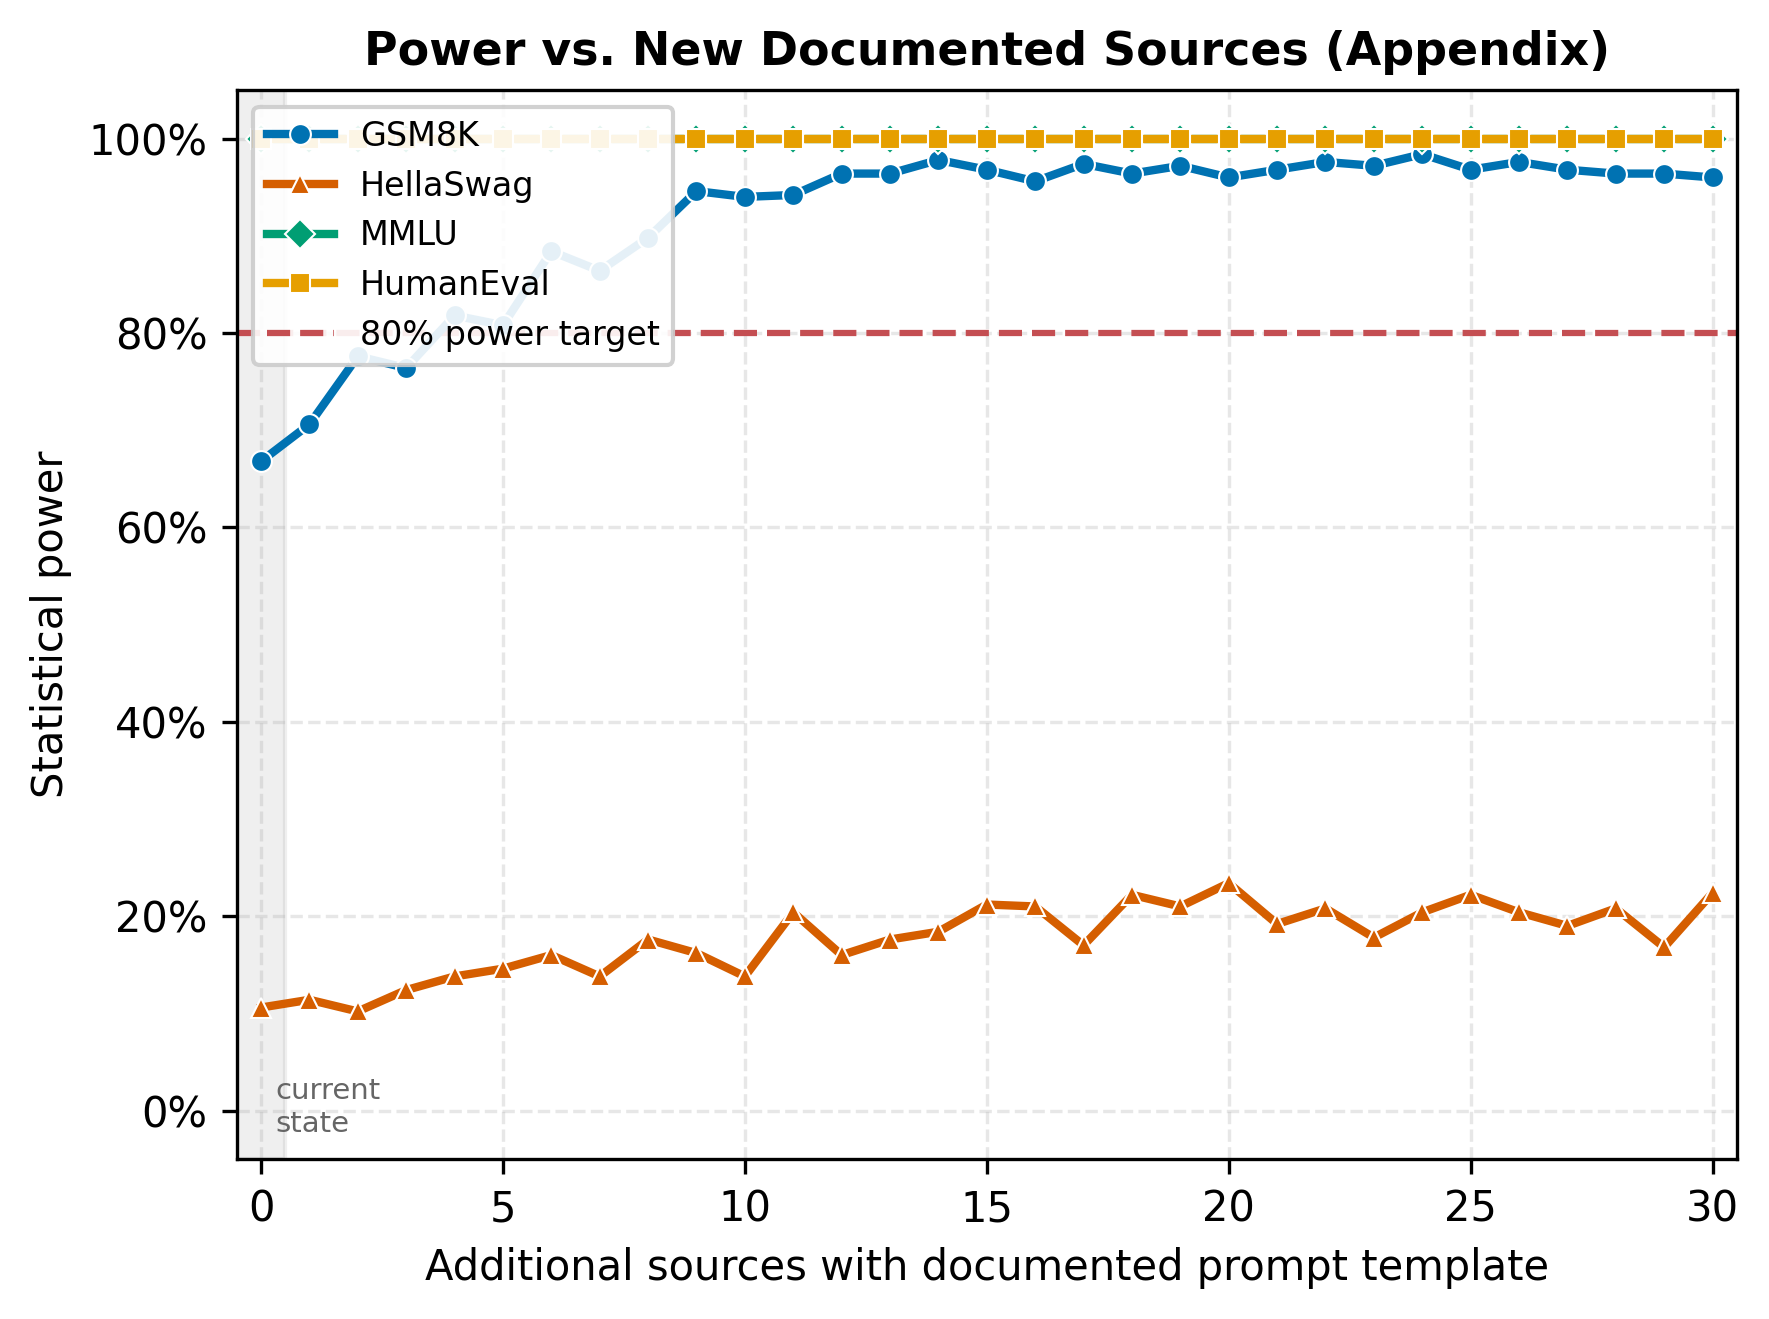
\includegraphics[width=\columnwidth]{fig8_appendix_power_vs_sources.png}
\caption{Power vs.\ number of additional documented sources, per benchmark.
MMLU reaches 80\% power at $\sim$7 new sources; GSM8K at $\sim$9;
HellaSwag and HumanEval remain under-powered at 30.}
\label{fig:projection_left}
\end{figure}

%% -------------------------------------------------------------------
\section{Power Simulation: Sources Needed for 80\% Power}
\label{app:power_sim}

Figure~\ref{fig:power_app} shows the power simulation previously
included in the main body; it is demoted here because the
coverage--power projection (Figure~\ref{fig:projection}) conveys the
same message in a more actionable form.

\begin{figure}[t]
\centering

\includegraphics[width=\columnwidth]{fig6_power_simulation.png}
\caption{Power simulation for the dominant methodology predictor per
benchmark. \emph{Left}: power as a function of $k$ sources at observed
effect sizes with $R^2 \pm 0.15$ uncertainty bands (shaded).
\emph{Right}: minimum sources for 80\% power. All effect sizes are from
pilot data.}
\label{fig:power_app}
\end{figure}

\end{document}